%!TEX root = /Users/stevenmartell/Documents/iSCAM-project/fba/Halibut/WRITEUP/Halibut.tex

\section{Simulation Model} % (fold)
\label{sec:simulation_model}
A detailed analytical description of the simulation model is provided in Appendix \ref{sec:model_description}.  The following is a summary description of specific model outputs that are used to describe the impacts of bycatch and wastage on halibut biomass, yield, spawning biomass and wastage, as well as, the corresponding size/age composition.  Ultimately, a decision table is constructed where the expected outcome (performance measure) is evaluated across alternative future states (good/bad recruitment, increasing/decreasing growth) for a series of alternative policy options.  The columns of this table represent alternative future states, and rows of the table correspond to different harvest policies. Assuming all future scenarios are equally likely, then the performance and sensitivity of alternative harvest polices can be easily compared.

\subsection{Overview of the simulation model} % (fold)
\label{sub:overview_of_the_simulation_model}
 Running a single realization of the simulation model consists of several steps that can be broken down into two periods: (1) initializing the model from 1996:2011, (2) future projections from 2012:2026.  Refer to Appendix \ref{sec:model_description} for detailed information on step (1).  Future projections in step (2) consists roughly 10 steps described by the following psuedo code:
\begin{enumerate}
	\item	Initialize future recruitment vector based on recruitment scenario
	\item	Project future weight at age based on growth scenario  (done in calcGrowth)
	\item	Future selectivity continues to be a function of length (done in calcSelectivities)
	\item	Loop from nyr to nyr+nyr\_proj
	\item	Calculate Ebio at the start of the year (EBio = N * sel * wa)
	\item	Apportion Ebio to management areas ($l$) based on 2011 apportionments
	\item	Calculate management area CEY as 0.215*EBio$_l$ or 0.16*EBio$_l$
	\item	Calculate the corresponding fishing rate ($f_{h,i,k}$)
	\item	Calculate Z and update total mortality.
	\item	Update numbers at age and return to 4) until end of projection years.
\end{enumerate}

Future recruitment is actually initialized in the year 2007, as halibut are roughly 6 years of age before they recruit to the fishery. Three alternative recruitment scenarios are explored, where future recruitment is based on the 25, 50 and 75th percentiles of the historical recruitment estimated between 1996 and 2006.
%Recruitment scenarios 
%lnRbar =17.93703
%w25 = -0.2928
%w50 =  0.1020
%w75 =  0.2399

Three alternative scenarios were also used to project future growth of halibut beyond 2011.  To simulate three alternative states of future growth a density-dependent relationship between cohort strength and the asymptotic length of males and females was developed.  To approximate future growth for each sex, a von Bertalanffy growth model was fit to the IPHC survey mean length-at-age data collected between 1996 and 2011 (Figure \ref{fig:FIGURES_figLengthAtAgeFit} a,b).  I then arbitrarily allow growth to vary by adjusting the asymptotic length of each cohort as a function of recruitment density. For example, if recruitment is roughly 2.7 times larger than the average recruitment, the the asymptotic length would decrease from 148 cm to 139 cm under density-dependent growth, and it would increase to 157 cm under inverse density-dependent growth (Figure \ref{fig:FIGURES_figLinf}).  

Converting numbers-at-age to weight-at-age, the allometric relationship $w_j= a l_j^b$ was used.  The scaling and power parameters ($a=9.321x10^{-6}$ and $b=3.16$) were taken from \cite{courcellesre}.  Note that the empirical weight-at-age data from the commercial catch versus the length-at-age data from the IPHC setline survey used in the IPHC assessment model are also plotted on Figures \ref{fig:FIGURES_figLengthAtAgeFit}cd. For the most part empirical weight-at-age is larger than the predicted weight-at-age from \cite{courcellesre}.  Attempts were made to estimate the corresponding allometric parameters from the empirical data; however, there was difficulty obtaining reasonable estimates from these two separate sources of information.  Log-log plots of these data do not reveal a linear relationship between the log-length and log-weight.  In fact, the male appear to shrink from 14 pounds at age-6 to less than 14 pounds at ages 7-10.  Therefore, all weight-at-age data in the simulation model are based on the allometric relationship from the \cite{courcellesre} study.
   
\begin{figure}[htbp]
	\centering
		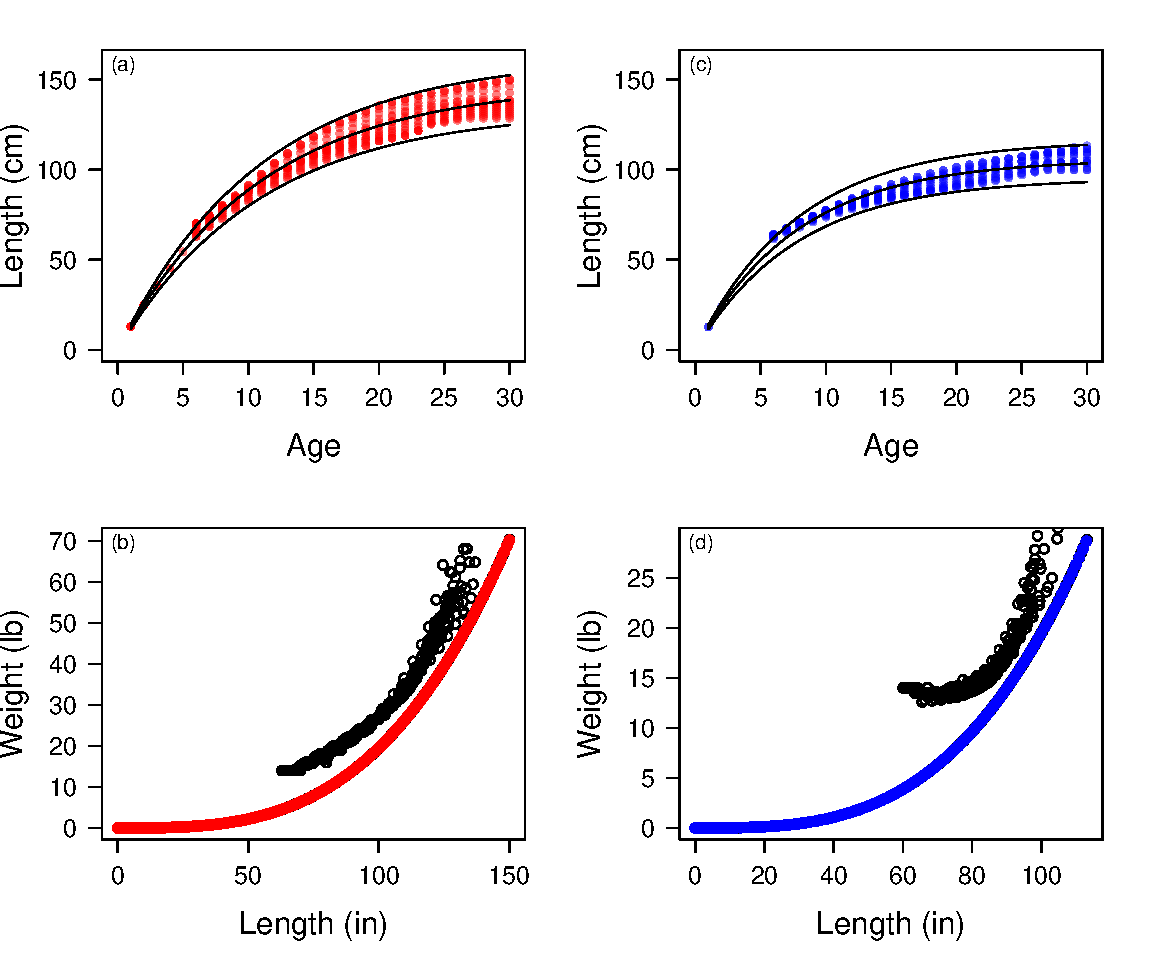
\includegraphics[width=0.9\textwidth]{../FIGURES/figLengthAtAgeFit.pdf}
	\caption{Observed mean length-at-age for female (a) and male (b) halibut in the IPHC research surveys between 1996 and 2011. Fitted lines are the von Bertalanffy growth model with the boundaries based on a 10\% coefficient of variation in the asymptotic length. Estimated parameters for females are $L_\infty=148.06$, $k=0.0915$, and for males $L_\infty=105.73$, $k=0.1275$. Panels c  (female) and d (male) show the length-weight relationship used in the model, along with the empirical catch weight-at-age data used in the IPHC assessment.}
	\label{fig:FIGURES_figLengthAtAgeFit}
\end{figure}

\begin{figure}[htbp]
	\centering
		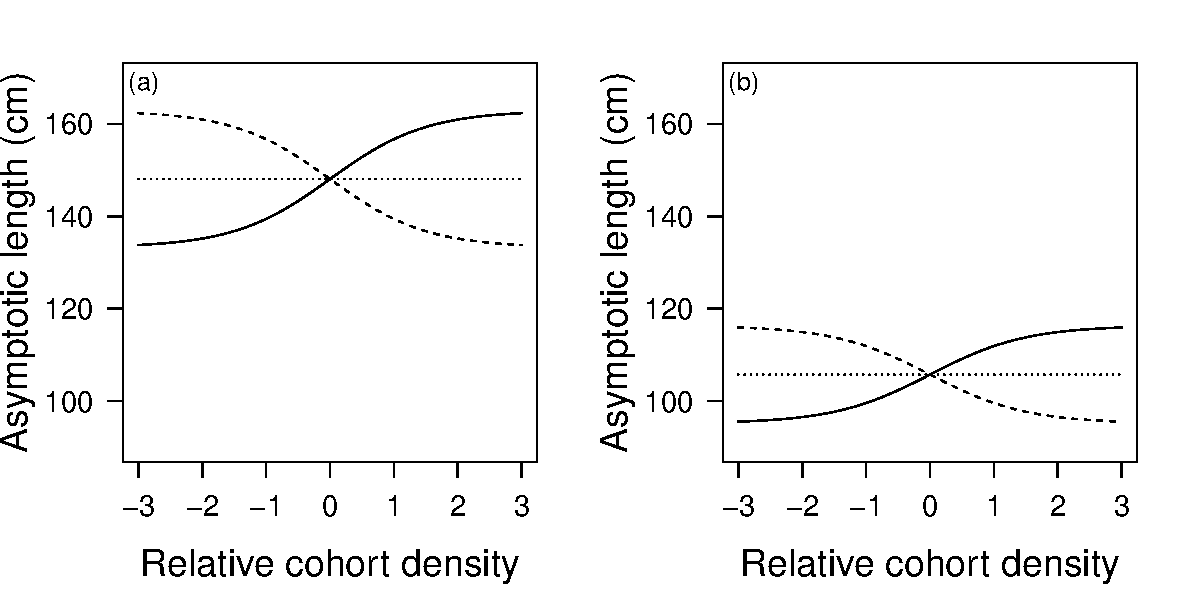
\includegraphics[width=0.9\textwidth]{../FIGURES/figLinf.pdf}
	\caption{Relationship between asymptotic length $l_\infty^{(h)}$ for females (a) and males (b) and cohort density. Under density-dependent growth, $l_\infty^{(h)}$ decreases with increasing density (dashed line), inverse density-dependent (solid line), and density independent (dotted line).  }
	\label{fig:FIGURES_figLinf}
\end{figure}

Selectivity in the simulation model is the exact same length-based selectivity that is used in the IPHC assessment.  The same piece-wise linear function that is used to convert mean length-at-age to age-based selectivity for the five different harvest categories in the simulation model (Firgure \ref{fig:FIGURES_fig:AgeSel}).  Overall males recruit to the various gears at much older ages due to slower growth of male halibut.
\begin{figure}[htbp]
	\centering
		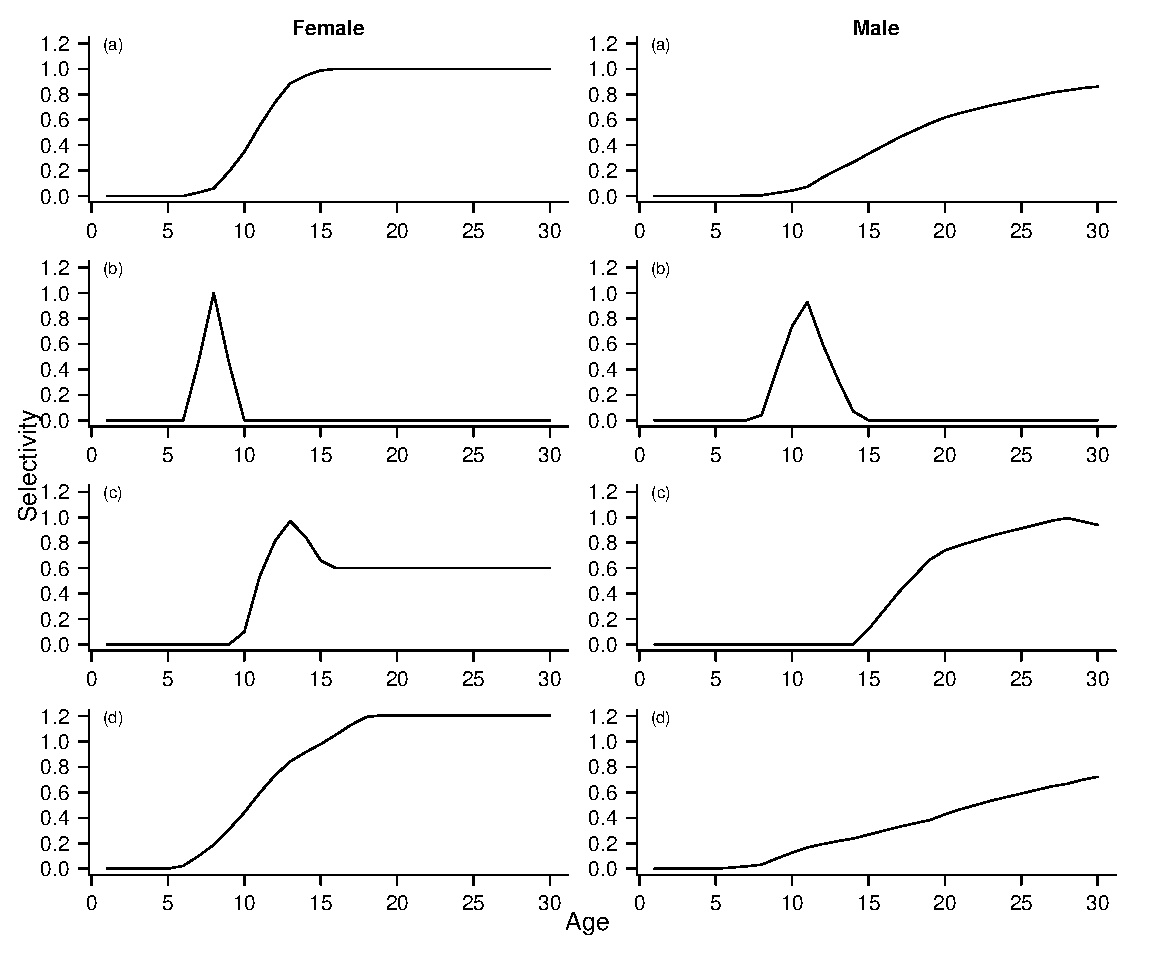
\includegraphics[width=0.8\textwidth]{../FIGURES/fig:AgeSel.pdf}
	\caption{Age-based selectivity coefficients for female and male halibut for the setline fishery (a), U32 (b), O32 (c), the recreational and personal use fisheries (d,e).}
	\label{fig:FIGURES_fig:AgeSel}
\end{figure}

Simulated exploitable biomass each year is based on the sum of products between the numbers-at-age,  weight-at-age, and selectivity-at-age for both sexes combined.  Apportionment of this coast-wide exploitable biomass to each of the statistical areas is based on the same apportionment scheme used by the IPHC staff in 2011.  The constant exploitable yield ($\mathrm{CEY}_{i,l}$) in year $i$ for  management area $l$ was based on the application of area-specific harvest rate of 0.215 (areas 2A-3A) and 0.161 (areas 3B-4CDE).
% subsection overview_of_the_simulation_model (end)
\subsection{Calculating setline fishery allocation} % (fold)
\label{sub:calculating_setline_fishery_allocation}
Annual allocations to the directed setline fishery in each of the areas are determined by first subtracting the expected bycatch/wastage from the area CEY.  To simulate the same procedure for each statistical area, annual directed setline allocation was calculated as:
\[ C_{i,k=1} = \mathrm{CEY}_{i,l} - \sum_{k=2}^{k=5} C_{i,k}, \]
where the catch allocations for gears other than the setline fishery ($k>1$) are determined \emph{a priori}.  The rule differes slightly for area $l$=2B where 88\% and 12\% of the allocation is given to the commercial and recreational fisheries, respectively.


% subsection calculating_setline_fishery_allocation (end)
\subsection{Calculating area specific fishing mortality rates} % (fold)
\label{sub:calculating_area_specific_fishing_mortality_rates}
A critical component of the simulation model is calculating the sex/age-specific fishing mortality rates from each of the major fisheries that target halibut or intercept them as bycatch.  The IPHC uses two terms to for the non-targeted mortality: (1) wastage, which is the catch of undersize fish, lost skates and loss at the rail of halibut in the directed fishery, and (2) bycatch which is the interception of halibut in non-targeted fishery including groundfish trawl, longline, trap, and pelagic trawl.

The catch equation used in the IPHC assessment model and in this simulation model assumes that both natural mortality and fishing mortality occur simultaneously.  This equation, also known as the Baranov catch equation, is given by:
\[
 C_{i,k} =\sum_h \sum_j \frac{N_{h,i,j} w_{h,i,j} f_{h,i,k} s_{h,i,j} (1-\exp(-Z_{h,i,j}))}{Z_{h,i,j}}
\]
For a given catch allocation $C_{i,k}$, the annual fishing mortality rate ($f_{h,i,k}$) for gear $k$ is solved for using an iterative method where it is assumed that the sex ratio of the catch is the same as the ratio of female:male vulnerable biomass.  This approach differs from the approach used in the IPHC assessment, where annual fishing mortality rates for females are treated as  latent variables and the male fishing mortality rate is proportional to the female fishing mortality rate.  The latter method could not be used in the simulation model  because it would require a catch allocation by sex.

For the directed setline fishery, the wastage component from this fishery is a combination of undersized fish and legal sized fish that are lost at the rail, or died.  To simulate this process, a joint probability model was developed to account for the wastage of undersized fish. The joint probability model is defined as:
\[
 v_{h,i,j,k} = s_{h,i,j,k}(r_{h,i,j,k}+(1-r_{h,i,j,k})d_{k}),
\]
where $v_{h,i,j,k}$ is the sex/age specific vulnerability to fishing from gear $k$ in year $i$, $s_{h,i,j,k}$ is the probability of capturing a fish of age $j$, $r_{h,i,j,k}$ is the retention probability (i.e., the probability of being greater than the size limit for a given age), and $d_{k}$ is the discard mortality rate associated with gear $k$.
% subsection calculating_area_specific_fishing_mortality_rates (end)

\subsection{Model outputs} % (fold)
\label{sub:model_outputs}

Summary equations for the simulated model output are presented in Table \ref{table:ModelOutputs}.  The simulated exploitable biomass ($EBio_i$) is the vulnerable biomass available to the commercial fishery \eqref{eqOutput:T1.1}, where $k=1$ denotes the selectivity for the commercial setline gear.  Annual spawning stock biomass ($SBio_i$) is based on the female component only ($h=1$) and the empirical weight-at-age data and the proportion mature $p_{h,j}$, \eqref{eqOutput:T1.2}.  Note that for both the exploitable biomass  in the IPHC assessment is based on the empirical weight-at-age data from the commercial catches and ranges from ages 6:20 from 1996:2001, and ages 6:25 in 2001:2011 period.  The commercial wastage in the simulation model is based only on the undersized fish that are discarded \eqref{eqOutput:T1.3}, where $s_{h,i,j,k=1}$ is the commercial age-specific selectivity (a function of fish length), $r_{h,k,j,k=1}$ is age-specific retention probability, and $d_{k=1}$ is the discard mortality rate for the commercial fishery and is assumed to be 0.17 for this study.  The commercial yield of legal sized fish is given by \eqref{eqOutput:T1.4}.

\begin{table}
	\caption{Summary calculations for model output}
	\label{table:ModelOutputs}
	\begin{center}
	\tableEq
	\begin{align}
		\hline \nonumber\\
		&\mbox{Exploitable Biomass}
		&EBio_i &= \sum_h \sum_{j=6}^{j=30} N_{h,i,j} w_{h,i,j} \exp(\nu_{h,i,j,k=1})\label{eqOutput:T1.1} \\
		%
		&\mbox{Spawning Biomass}
		&SBio_i &= \sum_{j=6}^{j=30} N_{h=1,i,j} w_{h=1,i,j} p_{h=1,j}\label{eqOutput:T1.2}\\
		%
		&\mbox{Commercial Wastage}
		&WBio_i &= \sum_h \sum_j \frac{N_{h,i,j}w_{h,i,j}f_{h,i,k=1}s_{h,i,j,k=1}(1-r_{h,i,j,k=1})d_{k=1}}
		{Z_{h,i,j}} \label{eqOutput:T1.3}\\
		%
		&\mbox{Commercial Yield}
		&YBio_i &= \sum_h \sum_j \frac{N_{h,i,j}w_{h,i,j}f_{h,i,k=1}s_{h,i,j,k=1} r_{h,i,j,k=1}}
		{Z_{h,i,j}}\label{eqOutput:T1.4}\\
		%
		&\mbox{Lost Yield}
		&LBio_i &= YBio_i^{(f_{k=2,3}=0)} - YBio_i \label{eqOutput:T1.5}\\
		%
		&\mbox{Bycatch Yield}
		&BBio_i &= \sum_h \sum_j \sum_{k=2}^{k=3}\frac{N_{h,i,j}w_{h,i,j}f_{h,i,k}s_{h,i,j,k} r_{h,i,j,k}}
		{Z_{h,i,j}}\label{eqOutput:T1.6}\\
		%
		&\mbox{Yield Loss Ratio}
		&YLR_i & = \frac{LBio_i}{BBio_i}\label{eqOutput:T1.7} \\
		\hline \nonumber
	\end{align}
	\normalEq
	\end{center}
\end{table}

To calculate the yield loss due to bycatch in non-directed fisheries, the simulation model was project forward in time where the only source of fishing mortality is the directed fishery (including deaths from wastage) and the recreational and personal use.  To do this, the bycatch allocations for the U32 and 032 fisheries were set to 0 and the corresponding fishing rates for these two gears are also determined to be 0 for all future projection years.  This simulation run is denoted as $YBio_i^{(f_{k=2,3}=0)}$.  The lost yield due to by catch is the difference between the commercial yields with and without bycatch fishing mortality \eqref{eqOutput:T1.5}.  Note also, that with no bycatch fishing mortality, the annual allocation to the commercial fishery is the total area $\mathrm{CEY}_{i,l}$ minus the recreational and personal use allocations:
\[ C_{i,k=1} = \mathrm{CEY}_{i,l} - \sum_{k=4}^{k=5} C_{i,k}. \]

% subsection model_outputs (end)

% section simulation_model (end)


































